\chapter{Autoregressive Model}

\paragraph{Motivating Example: MNIST} \mbox{}\\
Given a dataset $D$ of handwritten digits, each image has $28\times 28 = 784$ pixels. Each pixel is a binary variable. Goal is to learn a probability distribution $p(x) = p(x_1,...,x_{784}$ such that when we sample $x\sim p(x)$, x looks like a digit. 

\section{Model Structure}
We can pick an ordering of all random variable (e.g.: from top left corner to bottom right, raster scan). Now with chain rule, we have 
    \begin{align*}
        p(x_1,...,x_{784}) = p(x_1) p(x_2|x_1) \cdots p(x_n|x_1,...,x_{n-1})
    \end{align*}
We choose to use a series of function with parameter $\alpha^{(n)}$ to estimate. e.g.: 
    \begin{align*}
        p(x_1,...,x_{784}) = p(x_1; \alpha^{(1)}) p_{logit}(x_2|x_1; \alpha^{(2)}) \cdots p_{logit}(x_n|x_1,...,x_{n-1}; \alpha^{(n)})
    \end{align*}
    \begin{itemize}
        \item $p(X_1 = 1) =  \alpha^{(1)}$
        \item $p_{logit}(x_2=1|x_1,  \alpha^{(2)}) = \sigma( \alpha_0^{(2)} +  \alpha_1^{(2)}x_1)$
    \end{itemize}
    
    
\subsection{Example : Fully Visible Sigmoid Belief Netowrk (FVSBN)}
The conditional variable $x_i |x_1, ..., x_{i-1}$ are Bernoulli with parameters. The approximation function is just the logit function. 
    \begin{align*}
        \hat{x_i} = p(x_i=1|x_1,...,x_{i-1};\alpha^{(i)}) = \sigma(\alpha_0^{(i)} + \sum_{j=1}^{i-1}\alpha_j^{(i)}x_j)
    \end{align*}
We can evaluate the joint probability by just multiplying everything together
    \begin{align*}
        p(x_1,x_2,x_3,x_4) = p(x_1) * p(x_2|x_1) * p(x_3|x_1,x_2) \cdots
    \end{align*}
For sampling, we just do sequential sampling. Pick $x_1$ first, and then $x_2$ and so on. Overall, we need $1 + 2 + 3 +... n$, hence $O(n^2)$ number of parameter. 

\subsection{Example : Neural Autoregressive Density Estimation (NADE)}
For NADE, we use a one layer neural network to replace logistic regression as estimation. 
    \begin{align*}
        \hat{x}_i = p(x_i | x_1,...,x_{i-1}; A_i, c_i, \alpha_i, b_i) = \sigma(\alpha_i (A_i x_{<i} + c_i) + b_i)
    \end{align*}
    \begin{itemize}
        \item $A_i x_{<i} + c_i$: the layer calculation 
        \item in reality, we can tie the weight together. So $A_2$ has column $w_1$, then $A_3$, the network matrix for calculating $x_3$, will also have $w_1$, and an additional column $w_2$
        \item linear in $n$ in terms of weights 
    \end{itemize}


\subsection{Example: RENADE} 
For non-binary discrete random variable $X_i \in \{1, ..., K\}$, we can let $\hat{x}_i$ parameterize a categorical distribution. 
    \begin{align*}
        & h_i = \sigma (W_{<i} \cdot x_{<i} + c) \\
        & p(x_i|x_1,...,x_{i-1}) = Cat(p_i^{(1)},...,p_i^{(K)})\\
        & \hat{x}_i = (p_i^{(1)},...,p_i^{(K)}) = softmax(A_ih_i + b_i) \\
        & softmax(a) = (\frac{exp(a^{(1)})}{\sum exp(a^{(i)})}, ...,\frac{exp(a^{(k)})}{\sum exp(a^{(i)})})
    \end{align*}
For continuous random variable, we want to let $\hat{x}_i$ parameterize a continuous distribution, such as mixture of $K$ Gaussians, i.e.: 
    \begin{align*}
        & p(x_i | x_1, ..., x_{i-1}) = \sum_{j=1}^K \frac{1}{K} \mathcal{N}(\mu_i^j, \sigma_i^j)\\
        & h_i = \sigma(W_{<i} \cdot x_{<i} + c)\\
        & \hat{x_i} = (\mu_i^1, ..., \mu_i^K, \sigma_i^1,...,\sigma_i^K) = f(h_i)
    \end{align*}
    \begin{itemize}
        \item Note here $j$ is not power, just a notiation for parameters for $x_j$
        \item we can use exponential to ensure the stand deviation is positive.
    \end{itemize}

\subsection{Example: Masked Autoencoders for Distribution Estimation (MADE)}
An autoencoder has two part, an encoder $e(\cdot)$, such as $e(x) = \sigma(W^2(W^1x+b^1)+b^2)$, and a decoer $d(\cdot)$ such that $d(e(X))\approx x$. For loss function, we can use cross entroy for binary data $\sum_{x\in D} \sum_i -x_i log\hat{x}_i - (1-x_i)log(1-\hat{x}_i)$ and MSE for continuous data $\sum_{x\in D}\sum_i (x_i - \hat{x}_i)^2$. \\

Note a vanilla autoencoder is not a generative model. But we can modify the graph to make sure it corresponds to a valid Bayesian Network (DAG structure). For example, if the ordering is 1, 2, 3, then $\hat{x}_1$ can not depend on any input $x$, $\hat{x}_2$ can only depend on $x_1$, and etc.  \\

We can achieve use this by using mask to disallow certain paths. 
\begin{figure}[h]
    \centering
    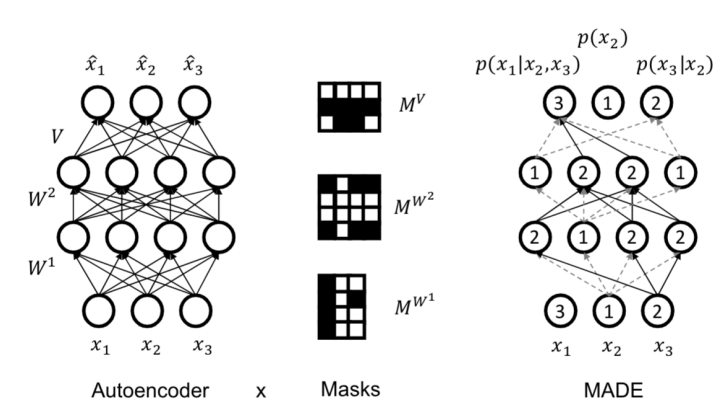
\includegraphics[width=12cm, height=10cm]{images/001_MADE.png}
    \caption{MADE Structure}
\end{figure}

In the structure of MADE, we first label all the input nodes $(1,2,3)$. Then for all the hidden nodes, we can arbitarily assign them a number $1 or 2$. If it is $1$, it means that this node only allow to take input from node with label $1$. If it is $2$, it means this node are allowed to take input from nodes with label $1$ and $2$. We then alter the mask for autoencoder to correspond to the disabled path. 



\subsection{Example: Character RNN} 
In the model $p(x_t|x_{1:t-1}; \alpha^t)$, the history $x_{1:t-1}$ keeps getting longer. One idea is to keep a summary and recursively update it. 

    \begin{align*}
        \textrm{Summary update rule: } h_{t+1} &= tanh(W_{hh}h_t + W_{xh} x_{t+1}) \\
        \textrm{Prediction: } o_{t+1} = W_{hy} h_{t+1} \\
        \textrm{Summary Initialization: } h_0 = b_0
    \end{align*}
    \begin{itemize}
        \item Hidden layer $h_t$ is a summary of the inputs seen till time $t$
        \item Output layer $o_{t-1}$ specifies parameters for conditional $p(x_t|x_{1:t-1})$
        \item Parameterized by $b_0$ (initialization), and matrices $W_{hh}, W_{xh}, W_{hy}$. Constant number of parameters w.r.t $n$. 
    \end{itemize}

\subsection{Additional Examples}
Some additional advanced example: 
    \begin{itemize}
        \item We can replace RNN with Transformer. It has attention mechanisms to adaptively focus on relevant context, and avoid recursive computation. It needs mased self-attention to preserve autoregressive structure 
        \item Pixel RNN uses LSTMs + masking 
        \item Pixel CNN uses CNN with masking. 
    \end{itemize}


\section{Training Generative Model with Maximum Likelihood Learning}
\paragraph{Setting} \mbox{}
Assume the domain is governed by some underlying distribution $P_{data}$. We are given a dataset $D$ of $m$ samples from $P_{data}$. The standard assumption is $iid$ samples. We are also given a family of models $M$, and our task is to learn some good model that defines a distribution $p_{\hat{M}}$. We treat it as a density estimation (learning the full distribution). 

\subsection{Kullback-LeiblerL Divergence}
KL Divergence can measure the distance between true distribution $p_{data}$ and the distribution from our fitted model family $q$. 
    \begin{align*}
        D(p||q) 
        & = \sum_{x} p(x) \log \frac{p(x)}{q(x)}\\
        &= E_{x\sim P}\left [ \log \frac{p(x)}{q(x)} \right ]\\
        &= E_{x\sim P}\left [ \log p(x) \right] - E_{x\sim P}\left[\log q(x) \right ]\\
    \end{align*}
    \begin{itemize}
        \item $d(p || q) \geq 0$ for all $p, q$
        \item $D(p||q) = 0$ iff $p = q$
        \item KL Divergence is asymmetric. I.e.: $D(p||q) \neq D(q||p)$
        \item Measures the expected number of extra bits required to describe samples from $p(x)$ using a code based on $q$ instead of $p$
        \item Notice at line 3 the first term is not dependent on $p_{data}$, so $\overset{argmin}{p_\theta} D(P_{data}||P_\theta)  =  \overset{argmin}{p_\theta} - E_{x \sim P_{data}}(\log p_\theta(x)) =  \overset{argmax}{p_\theta} E_{x \sim P_{data}}(\log p_\theta(x))$
        \item i.e.: We ask $P_{\theta}$ to assign the high probability to instances sampled from $P_{data}$, this is a maximum likelihood estimation. 
    \end{itemize}
\subsubsection{Using Jensen Inequality to Prove Non-negative of KL Divergence} 
    \begin{align*}
        D(p||q) 
        & = \sum_{x} p(x) \log \frac{p(x)}{q(x)}\\
        &= E_{x\sim P}\left [ \log \frac{p(x)}{q(x)} \right ] \\
        &= E_{x\sim P}\left [ -\log \frac{q(x)}{p(x)} \right ] \\
        &\geq - \log E_{x\sim P}\left [\frac{q(x)}{p(x)} \right ] \tag{Concavity of Log function} \\
        &= - \log \left(    \sum_x p(x) \frac{q(x)}{p(x)}   \right) \\
        &= - \log \left(    \sum_x q(x)  \right) \\
        &= - \log \left( 1)  \right) \\
        &= 0
    \end{align*}

\subsection{Maximum Likelihood}
Because we don't know $P_{data}$, we have to appxomiate the expected log-likelihood $E_{x\sim P_{data}}[\log P_\theta(x)]$ with the empirical log-likelihood: 
    \begin{align*}
        E_{D}[\log P_\theta (x)] = \frac{1}{|D|}\sum_{x\in D} log P_\theta(x)
    \end{align*}
So the maximum likelihood learning is 
    \begin{align*}
        \overset{max}{P_\theta} \frac{1}{|D|}\sum_{x\in D} log P_\theta(x)
    \end{align*}
This is equivalent to getting a distribution to assign high probability to the data (notice if we take the log on both side in below equation, we get our original objective) 
    \begin{align*}
        P_\theta(x^{(1)}, x^{(2)}, ..., x^{(m)}) = \prod_{x\in D} P_\theta(x) \\
    \end{align*}
    

\subsection{Monte Carlo Estimation}
We can use Monte Carlo Estimation to find the estimate of a function w.r.t a distribution when we don't know the distribution and only have samples from it. 
    \begin{enumerate}
        \item Express the quantity of interest as the expected value of a random variable: $E_{x\sim P}[g(x)] = \sum_x g(x) p(x)$
        \item Generate $T$ samples from the distribution $P$ with respect to which the expectation was taken 
        \item estimate the expected value from the sampling using $\hat{g}(x^1, ..., x^T) \overset{\triangle}{=} \frac{1}{T} \sum_{t=1}^T g(x^t)$
    \end{enumerate}
    \begin{itemize}
        \item Notice here $\hat{g}$ is the a random variable. 
        \item $\hat{g}$ is unbiased. i.e.: $E_p[\hat{g}] = E_p[g(x)]$
        \item By law of large numbers, $\hat{g}$ converges 
        \item Its variance is $\frac{V_p[g(x)]}{T}$. So as sample increases, the variance will decrease. 
    \end{itemize}
    
\subsection{MLE Scoring for Autoregressive Model}
Given an autoregressive model with $n$ variables and factorization, for a single $x$ sample, we can write it's probability as  
    \begin{align*}
        p_\theta(x) = \prod_{i=1}^{n} p_{neural}(x_i | x_{<i} ; \theta_i)
    \end{align*}
So the overall likelihood of the entire dataset is 
    \begin{align*}
        & L(\theta, D) = \prod_{j=1}^{m} P_\theta(x^{(j)}) = \prod_{j=1}^{m} \prod_{i=1}^{n} p_{neural}(x^{(j)}_i | x^{(j)}_{<i} ; \theta_i) \\
        & l(\theta) = \sum_{j=1}^{m} \sum_{i=1}^{n} \log p_{neural}(x^{(j)}_i | x^{(j)}_{<i} ; \theta_i)
    \end{align*}
We then use numerical solution (SGD) to find the max of this likelihood or the log likelihood. 
    \begin{itemize}
        \item Notice that for a specific $\theta_i$, say $\theta_t$, $\nabla_{\theta_t}l(\theta) = \sum_{j=1}^m \nabla_{\theta_t}\sum_{i=1}^{n} \log p_{neural}(x^{(j)}_i | x^{(j)}_{<i} ; \theta_i) = \sum_{j=1}^m \nabla_{\theta_t} \log p_{neural}(x^{(j)}_t | x^{(j)}_{<t} ; \theta_t)$. Hence the parameters for the $t'$ th conditional parameters only appears in the $t'$th conditional. Without parameter sharing, we are essentially optimizing each conditional parameter $\theta_i$ separately. 
    \end{itemize}
What if $m = |D|$ is huge, we can use SGD instead of GD
    \begin{align*}
        \nabla_\theta(l(\theta)) 
        &=  \sum_{j=1}^{m} \sum_{i=1}^{n} \nabla_\theta \log p_{neural}(x^{(j)}_i | x^{(j)}_{<i} ; \theta_i)\\
        &= m * \sum_{j=1}^{m} * \frac{1}{m} \sum_{i=1}^{n} \nabla_\theta \log p_{neural}(x^{(j)}_i | x^{(j)}_{<i} ; \theta_i)\\
        &= m * E_{x^{(j)} \sim D} \left[ \sum_{i=1}^{n} \nabla_\theta \log p_{neural}(x^{(j)}_i | x^{(j)}_{<i} ; \theta_i)  \right]\\
        & \textrm{Estimate the expectation by taking a sample from the dataset and evaluate the gradient}
    \end{align*}


\subsection{Overfitting} 
Empirical risk minimization can easily overfit the data. The extreme example is that the model memerize the data, and have uniform probability over the training set. So we typically restrict the hypothesis space of distribution  that we search over or add the regularization term to bias the model to simpler structure. 
    \begin{itemize}
        \item Smaller neural networks with less parameters 
        \item weight sharing 
        \item conditional independence assumption 
        \item Regularization 
    \end{itemize}